\chapter{Escenario 7: obtención de datos}
\sourcebadge{Reconstruido desde el índice; los datos adicionales son ficticios y se identifican como simulados.}

La fuente original contiene 3.000 incidentes. Su copia de trabajo fue verificada con SHA-256. El valor se presenta en dos segmentos para conservar la legibilidad:

\begin{center}\small\ttfamily
814F3E5D8CF983A86BC125EC9C8461E\\
3728C91DDCE1CFE8A5518ABD7A53CDC17
\end{center}

El archivo no se modifica durante el pipeline.

La simulación con semilla 25022 produce 6.000 eventos y 2.000 encuestas entre enero y diciembre de 2025. Cada evento contiene fecha, sede, rol, módulo, duración, resultado, código de error, característica ISO, semilla y bandera \texttt{simulated}.

\begin{figure}[H]\centering
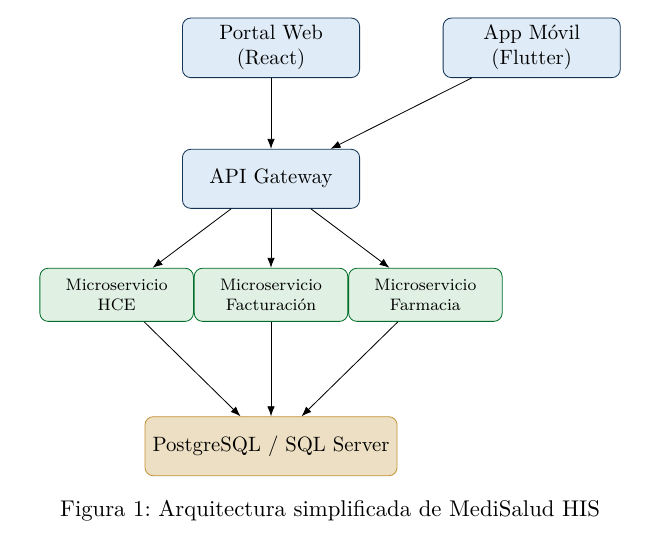
\includegraphics[width=0.9\textwidth]{figures/architecture.png}
\caption{Arquitectura simplificada del caso. Fuente: Documento Padre.}
\end{figure}
